\documentclass{article}
\usepackage{graphicx}
\usepackage{wrapfig}
\usepackage{subcaption}
\usepackage[margin=1in]{geometry}
\usepackage{amsmath} % or simply amstext
\usepackage{siunitx}
\usepackage{booktabs}
\usepackage[export]{adjustbox}
\newcommand{\angstrom}{\textup{\AA}}
\newcommand{\colormap}{jet}  % colorbar to use
\usepackage{cleveref}
\usepackage{booktabs}
\usepackage{gensymb}
\usepackage{float}
\usepackage{xr}

\externaldocument[M-]{Draft}

\renewcommand{\thefigure}{S\arabic{figure}}
\renewcommand{\thesection}{S\arabic{section}}
\renewcommand{\thepage}{S\arabic{page}}
\renewcommand{\thetable}{S\arabic{table}}

\title{Supporting Information: Time Series Modeling of Solute Transport in an H\textsubscript{II} 
Phase Lyotropic Liquid Crystal Membrane}
\author{Benjamin J. Coscia \and Michael R. Shirts} 

\begin{document}

  \maketitle
  \graphicspath{{./supporting_figures/}}
  \bibliographystyle{ieeetr}
  
  \section{Setup and analysis scripts}\label{section:python_scripts}

  All python and bash scripts used to set up systems and conduct post-simulation trajectory
  analysis are available online at \texttt{https://github.com/shirtsgroup/LLC\_Membranes}.
  Documentation for the \texttt{LLC\_Membranes} repository is available at
  \texttt{https://llc-membranes.readthedocs.io/en/latest/}. Table~\ref{table:python_scripts}
  provides more detail about specific scripts used for each type of analysis performed in
  the main text.

  \begin{table}[htb!]
  \centering
  \newcolumntype{A}{ >{\centering\arraybackslash} m{2.5in} }
  \newcolumntype{B}{ >{\centering\arraybackslash} m{0.75in} }
  \newcolumntype{C}{m{2.75in}}
  \begin{tabular}{|A|B|C|}
  \hline
  \textbf{Script Name} & \textbf{Section} & ~~~~~~~~~~~~~~~~~~~~~\textbf{Description} \\
  \hline

  % mimic this
  \texttt{/setup/param.sh} & 2.1 & Parameterize liquid
  crystal monomers and solutes with GAFF \\ \hline

  \end{tabular}

  \caption{The first column provides the names of the python scripts available in
  the \texttt{LLC\_Membranes} GitHub repository that were used for system setup and
  post-simulation trajectory analysis. Paths preceding script names are relative to the
  \texttt{LLC\_Membranes/LLC\_Membranes} directory. The second columns lists the section in the main
  text where the output or usage of the script is first described. The third column
  gives a brief description of the purpose of each script.
  }~\label{table:python_scripts}

  \end{table}

  \section{Choosing a transport model}\label{section:transport_model_selection}

  We used the toolbox created by Meroz and Sokolov in order to justify our
  choice of transport model.\cite{meroz_toolbox_2015} The solutes in our systems
  exhibit anomalous transport properties characteristic of a Continuous Time
  Random Walk (CTRW). 

  \subsection*{Mean Squared Displacement}

  The general form of a mean squared displacement (MSD) curve is:
  \begin{equation}
	\langle x^2(t) \rangle \sim t ^ \alpha
	\label{eqn:msd}
  \end{equation}
  For brownian motion, $\alpha = 1$ and the MSD is linear. When $\alpha \neq
  1$, the particle of interest exhibits anomalous diffusion. Values of $\alpha$
  greater than 1 give rise to superdiffusion, while values of $\alpha$ less than
  1 give rise to subdiffusion.

  We can calculate the ensemble-averaged MSD curve by averaging the MSDs of
  each particle trajectory, where each MSD is calculated using:
  \begin{equation}
	\delta^2(t) = \| \mathbf{r}(t) - \mathbf{r}(0) \|^2
	\label{eqn:ensemble_msd}
  \end{equation}
  where $\|\cdot\|$ represents the Euclidean norm. 

  The mean squared displacement of solutes in our model is a non-linear
  function of time, with $\alpha < 1$ which is indicative of anomalous
  subdiffusion. Figure \ref{fig:msd_power_law}a plots the ensemble-averaged MSD
  curve for 24 ethanol molecules diffusing in a 10 wt\% water H\textsubscript{II}
  LLC membrane system. We fit a power law of the form $Ae^{\alpha}$ to the MSD
  curve. We performed 2000 bootstrap trials by randomly sampling 24 MSD curves
  with replacement from the 24 total ethanol MSD curves. The bootstrapped average
  value of $\alpha$ is 0.75 for this system. 
 
  \begin{figure}[!htb]
  \centering
% Generated with : msd.py -t PR_nojump.xtc -g PR.gro -r ETH -ensemble -power_law -a z -nboot 2000
% in directory: /home/bcoscia/Documents/Gromacs/Transport/NaGA3C11/ETH/10wt
  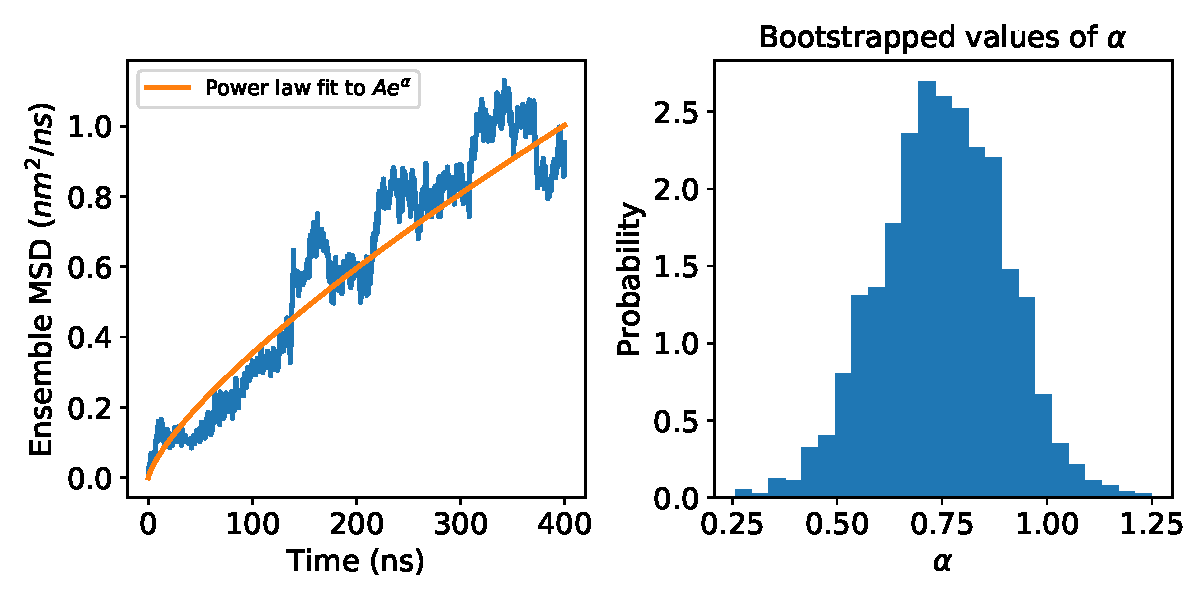
\includegraphics[width=0.8\linewidth]{msd_power_law.pdf}
  \caption{(a) We fit a curve with the form of Equation~\ref{eqn:msd} to the
	  ensemble-averaged MSD curve. (b) The average value of $\alpha$, obtained using
	  fits to MSDs calculated from bootstrapped ensembles, is less than 1 suggesting
	  that ethanol molecules in our model exhibit subdiffusive
	  behavior.}\label{fig:msd_power_law}
  \end{figure}

  \subsection*{Ergodicity}

  The ergodicity of a system can help us narrow down the possible anomalous
  diffusion mechanisms. In an ergodic system, the time-averaged behavior of an
  observable should yield the same result as the ensemble average of the same
  observable. Examples of anomalous diffusion processes that are ergodic include
  random walks on fractals (RWF) and fractional brownian motion (FBM).
  Non-ergodic systems generally give rise to CTRWs with the possibility of
  combination with a RWF and/or FBM.\cite{meroz_toolbox_2015} 

  We tested the ergodicity of our system by comparing the ensemble-averaged
  and time-averaged MSD curves. We calculated the MSD of each ethanol trajectory
  using Equation~\ref{eqn:ensemble_msd} and a time-averaged algorithm: 
  \begin{equation}
	\delta^2(t) = \dfrac{1}{N-t} \sum_{i=0}^{N-t-1} \| \mathbf{r}(i + t) - \mathbf{r}(i) \|^2
  \end{equation}
  where N is the total number of simulation frames, and t represents the length
  of subinterval or number of frames per subinterval. We averaged the MSD curves
  from each trajectory in order to create final MSD plots.

  The ethanol molecules exhibit non-ergodic behavior because their
  time-averaged and ensemble-averaged MSDs do not agree with each other
  (Figure~\ref{fig:ethanol_msd_comparison}). We validated our analysis using a 1
  ns simulation of a box of tip3p water molecules. As expected, since the
  particles exhibit Brownian motion, the time-averaged and ensemble-averaged MSDs
  agree with each within error (Figure~\ref{fig:water_box_msd_comparison}).

  \begin{figure}[!htb]
  \centering
  \begin{subfigure}{0.45\textwidth}
% Generated with : msd.py -t PR_nojump.xtc -g PR.gro -r ETH -compare -nboot 2000 -a z
% in directory: /home/bcoscia/Documents/Gromacs/Transport/NaGA3C11/ETH/10wt
  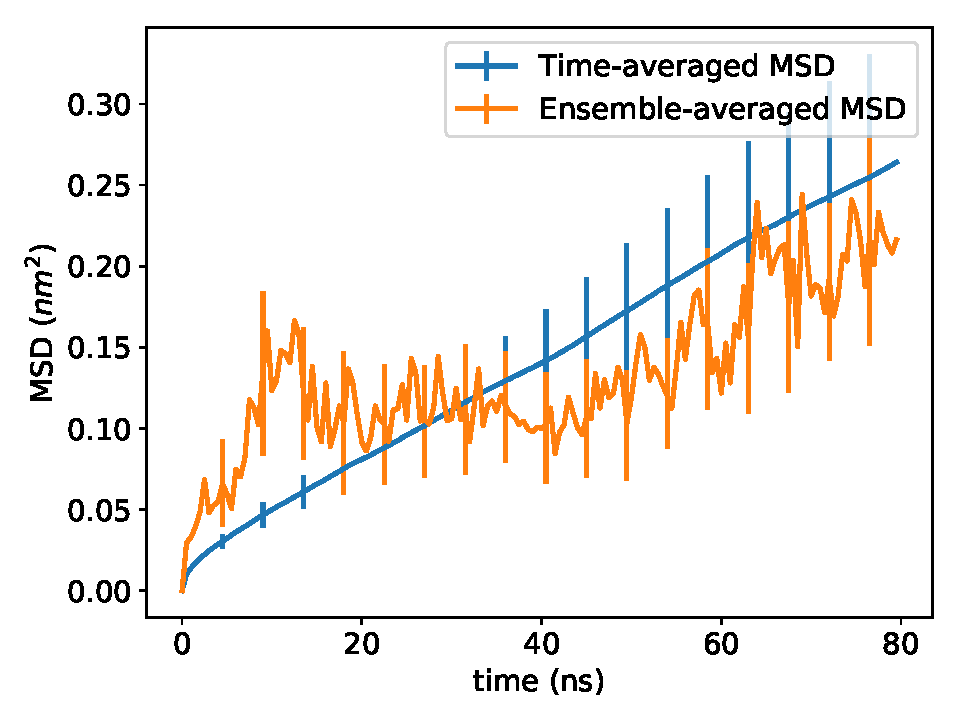
\includegraphics[width=\textwidth]{ethanol_msd_comparison.pdf}
  \caption{}\label{fig:ethanol_msd_comparison}
  \end{subfigure} 
  \begin{subfigure}{0.45\textwidth}
% Generated with msd.py -t traj_nojump.xtc -g npt.gro -r SOL -compare --fracshow 0.4 -nboot 2000 -a z
% in directory: /home/bcoscia/Documents/Gromacs/Transport/Solvent/solvent_boxes/pure_water
  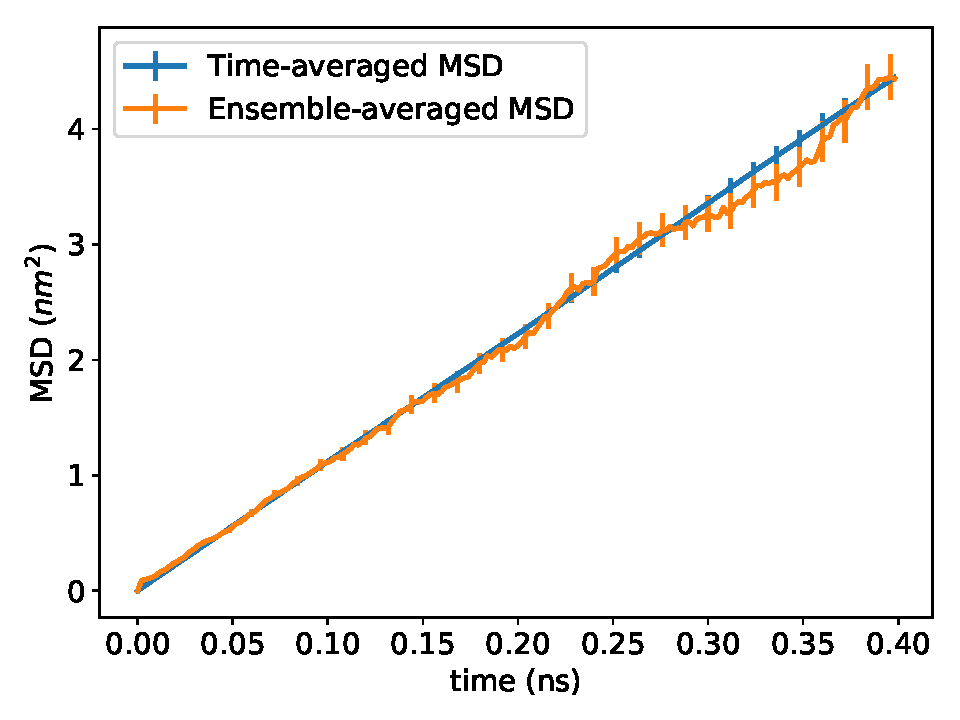
\includegraphics[width=\textwidth]{water_box_msd_comparison.pdf}
  \caption{}\label{fig:water_box_msd_comparison}
  \end{subfigure} 
  \caption{(a) The time-averaged and the ensemble-averaged MSDs for ethanol in
	  an H\textsubscript{II} nanopore are not in agreement, implying non-ergodicity.
	  (b) A box of tip3p water molecules is expected to be ergodic and it is shown to
	  be true here because both MSDs are in agreement. }\label{fig:msd_comparison}
  \end{figure}

  \subsection*{Autocorrelation of steps}

% From Sokolov paper: "Assigning different waiting times τ i to each step, and assuming that the
% steps are uncorrelated as in a regular RW, gives rise to the CTRW model" -- I
% might need to check autocorrelation of steps lengths when a hop occurs rather
% than every time step. Not sure if there is enough data for that, but could check 
% a particularly hoppy trajectory after longer simulation.


  Based on the previous two sections, our model can likey be studied as a CTRW. 
  However, it is still possible that our CTRW model might also be convoluted with
  an FBM or a RWF process. In a pure CTRW, the steps are uncorrelated. 
  Both FBM and RWF exhibit anti-correlated steps. 

  The steps in our system are not correlated. We showed this by calculating the
  autocorrelation function (ACF) of the step lengths in the $z$-direction. The
  ACF of a representative trajectory is shown in Figure~\ref{fig:eth_autocorrelation}.  
  
  \begin{figure}[!htb]
  \centering
% Generated with brownian_test.py -t PR_nojump.xtc -g PR.gro -r ETH (and appropriate uncommenting -- need to rework that script)
% in directory: /home/bcoscia/Documents/Gromacs/Transport/NaGA3C11/ETH/10wt
  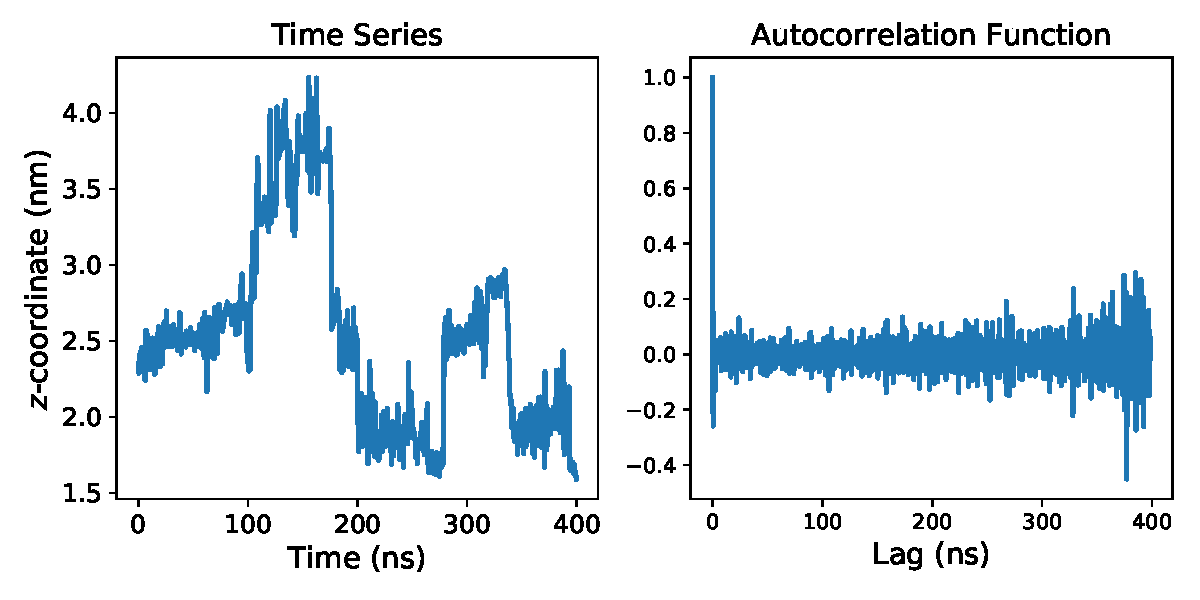
\includegraphics[width=0.8\textwidth]{eth_autocorrelation.pdf}
  \caption{The autocorrelation function (right) of a representative ethanol
	   center of mass $z$-coordinate trajectory (left) almost immediately decays to zero,
	   indicating a complete loss of memory of it's previous position. Noise increases
	   at large time lags due to decreased sampling.}\label{fig:eth_autocorrelation}
  \end{figure}
  
  \subsection*{Simulating Fractional L\'evy Motion}\label{section:sFLM}
  
  We simulated sFLM.

  \clearpage
  \bibliography{transport}

\end{document}
